\documentclass[aspectratio=169]{beamer}
\setbeamertemplate{navigation symbols}{}
\usepackage{color,amsmath,comment, subfigure}
\usepackage{booktabs}
\usepackage{url}

%\setbeameroption{show notes}

%%%%%%%%%%%%%%%%%%%%%%%%%%
\title[]{Lecture 3: More on the small world problem\\and some history}
\author[]{Sociology 204: Social Networks, Spring 2021}
\institute[]{Matthew J. Salganik}
\date[]{
2/3: Random graphs

\vfill

\begin{flushleft}
\vspace{0.7in}

\includegraphics[width=0.05\textwidth]{figures/cc.png}
\end{flushleft}
}

\begin{document}
%%%%%%%%%%%%%%%%%%%%%%%%%%%
\frame{\titlepage}
%%%%%%%%%%%%%%%%%%%%%%%%%%%
\begin{frame}

\begin{center}
\begin{columns}
\begin{column}{0.4\textwidth}
Empirical approach\\(Harvard approach)
\end{column}
\begin{column}{0.2\textwidth}
vs.
\end{column}
\begin{column}{0.4\textwidth}
Modeling approach\\(MIT approach)
\end{column}
\end{columns}
\end{center}

\end{frame}
%%%%%%%%%%%%%%%%%%%%%%%%%%%
\begin{frame}

\begin{center}
\begin{columns}
\begin{column}{0.4\textwidth}
Empirical approach\\(Harvard approach)
\end{column}
\begin{column}{0.2\textwidth}
vs.
\end{column}
\begin{column}{0.4\textwidth}
\textcolor{blue}{Modeling approach\\(MIT approach)}
\end{column}
\end{columns}
\end{center}

\end{frame}
%%%%%%%%%%%%%%%%%%%%%%%%%%%%
\begin{frame}

\begin{itemize}
\item What is the point of mathematical models?
\pause
\item How will we work with mathematical models in this class?
\end{itemize}

\note{
Billard balls, physics

}

\end{frame}
%%%%%%%%%%%%%%%%%%%%%%%%%%%
\begin{frame}

Erdos - Renyi Model

\note{
simplest possible model, draw a bunch of nodes on the board, throw down edges.  Giant component forms in a strange way

As you add edges the giant component does not grow linearly.  We will see things like this throughout the course: ice $\rightarrow$ water $\rightarrow$ steam

What is a mathematical model? Why is it useful?  When can it lead us astray?
}

\end{frame}
%%%%%%%%%%%%%%%%%%%%%%%%%%%
\begin{frame}

Demo

\vfill
\url{http://www.netlogoweb.org/launch\#http://ccl.northwestern.edu/netlogo/models/models/Sampl\%20Models/Networks/Giant\%20Component.nlogo}

\note{
run demo, with small number of nodes and watch giant component form, then reset with max number of nodes and re-run, but this time lets pretend these are Princeton students and the edges between then are sexual relationships.  If two people are not in the same component then they cannot spread STDs to each other.  

Is this a good model for friendship network at Princeton?  Why not? THINK - PAIR - SHARE\\
Possible answers: Not all ties are equally likely; timing; heterogeneity in degree distribution.
}

\end{frame}
%%%%%%%%%%%%%%%%%%%%%%%%%%%
\begin{frame}

We all get connected very quickly . . . 

\note{
Connection matters because things can spread
}

\end{frame}
%%%%%%%%%%%%%%%%%%%%%%%%%%%%
\begin{frame}

Is this is a good model for the social network at Princeton?\\
\pause
No. Not everyone is equally likely to be connected.

\end{frame}
%%%%%%%%%%%%%%%%%%%%%%%%%%%%
\begin{frame}

Network models
\begin{itemize}
\item Erdos-Reyni (dyadic)
\pause
\item Rappaport (triadic), wants the balance between randomness and order
\end{itemize}

\note{
Enter Rapoport\\
In Erdos-Reyni unit is dyad, Rapoport introduces the triad (Simmel said triads is where sociology begins)\\
Triadic closure bias a - b - c implies c - a (random biased nets)\\
Allows network to evolve over time, but runs into data and computing problems\\
How do you start? with random graph and fill in edges?  leads to completely connected network.  Duncan and I worked on this problem for one whole summer and got nowhere.\\

The main idea here is the \textbf{balance between order and randomness}.  This will be key for understand the small world\\
Point out difference between\\
\begin{itemize}
\item dynamics of networks
\item dynamics on networks
\end{itemize}

Rapaport's idea useful 50 years later  
}

\end{frame}
%%%%%%%%%%%%%%%%%%%%%%%%%%%
\begin{frame}

\begin{figure}
\centering
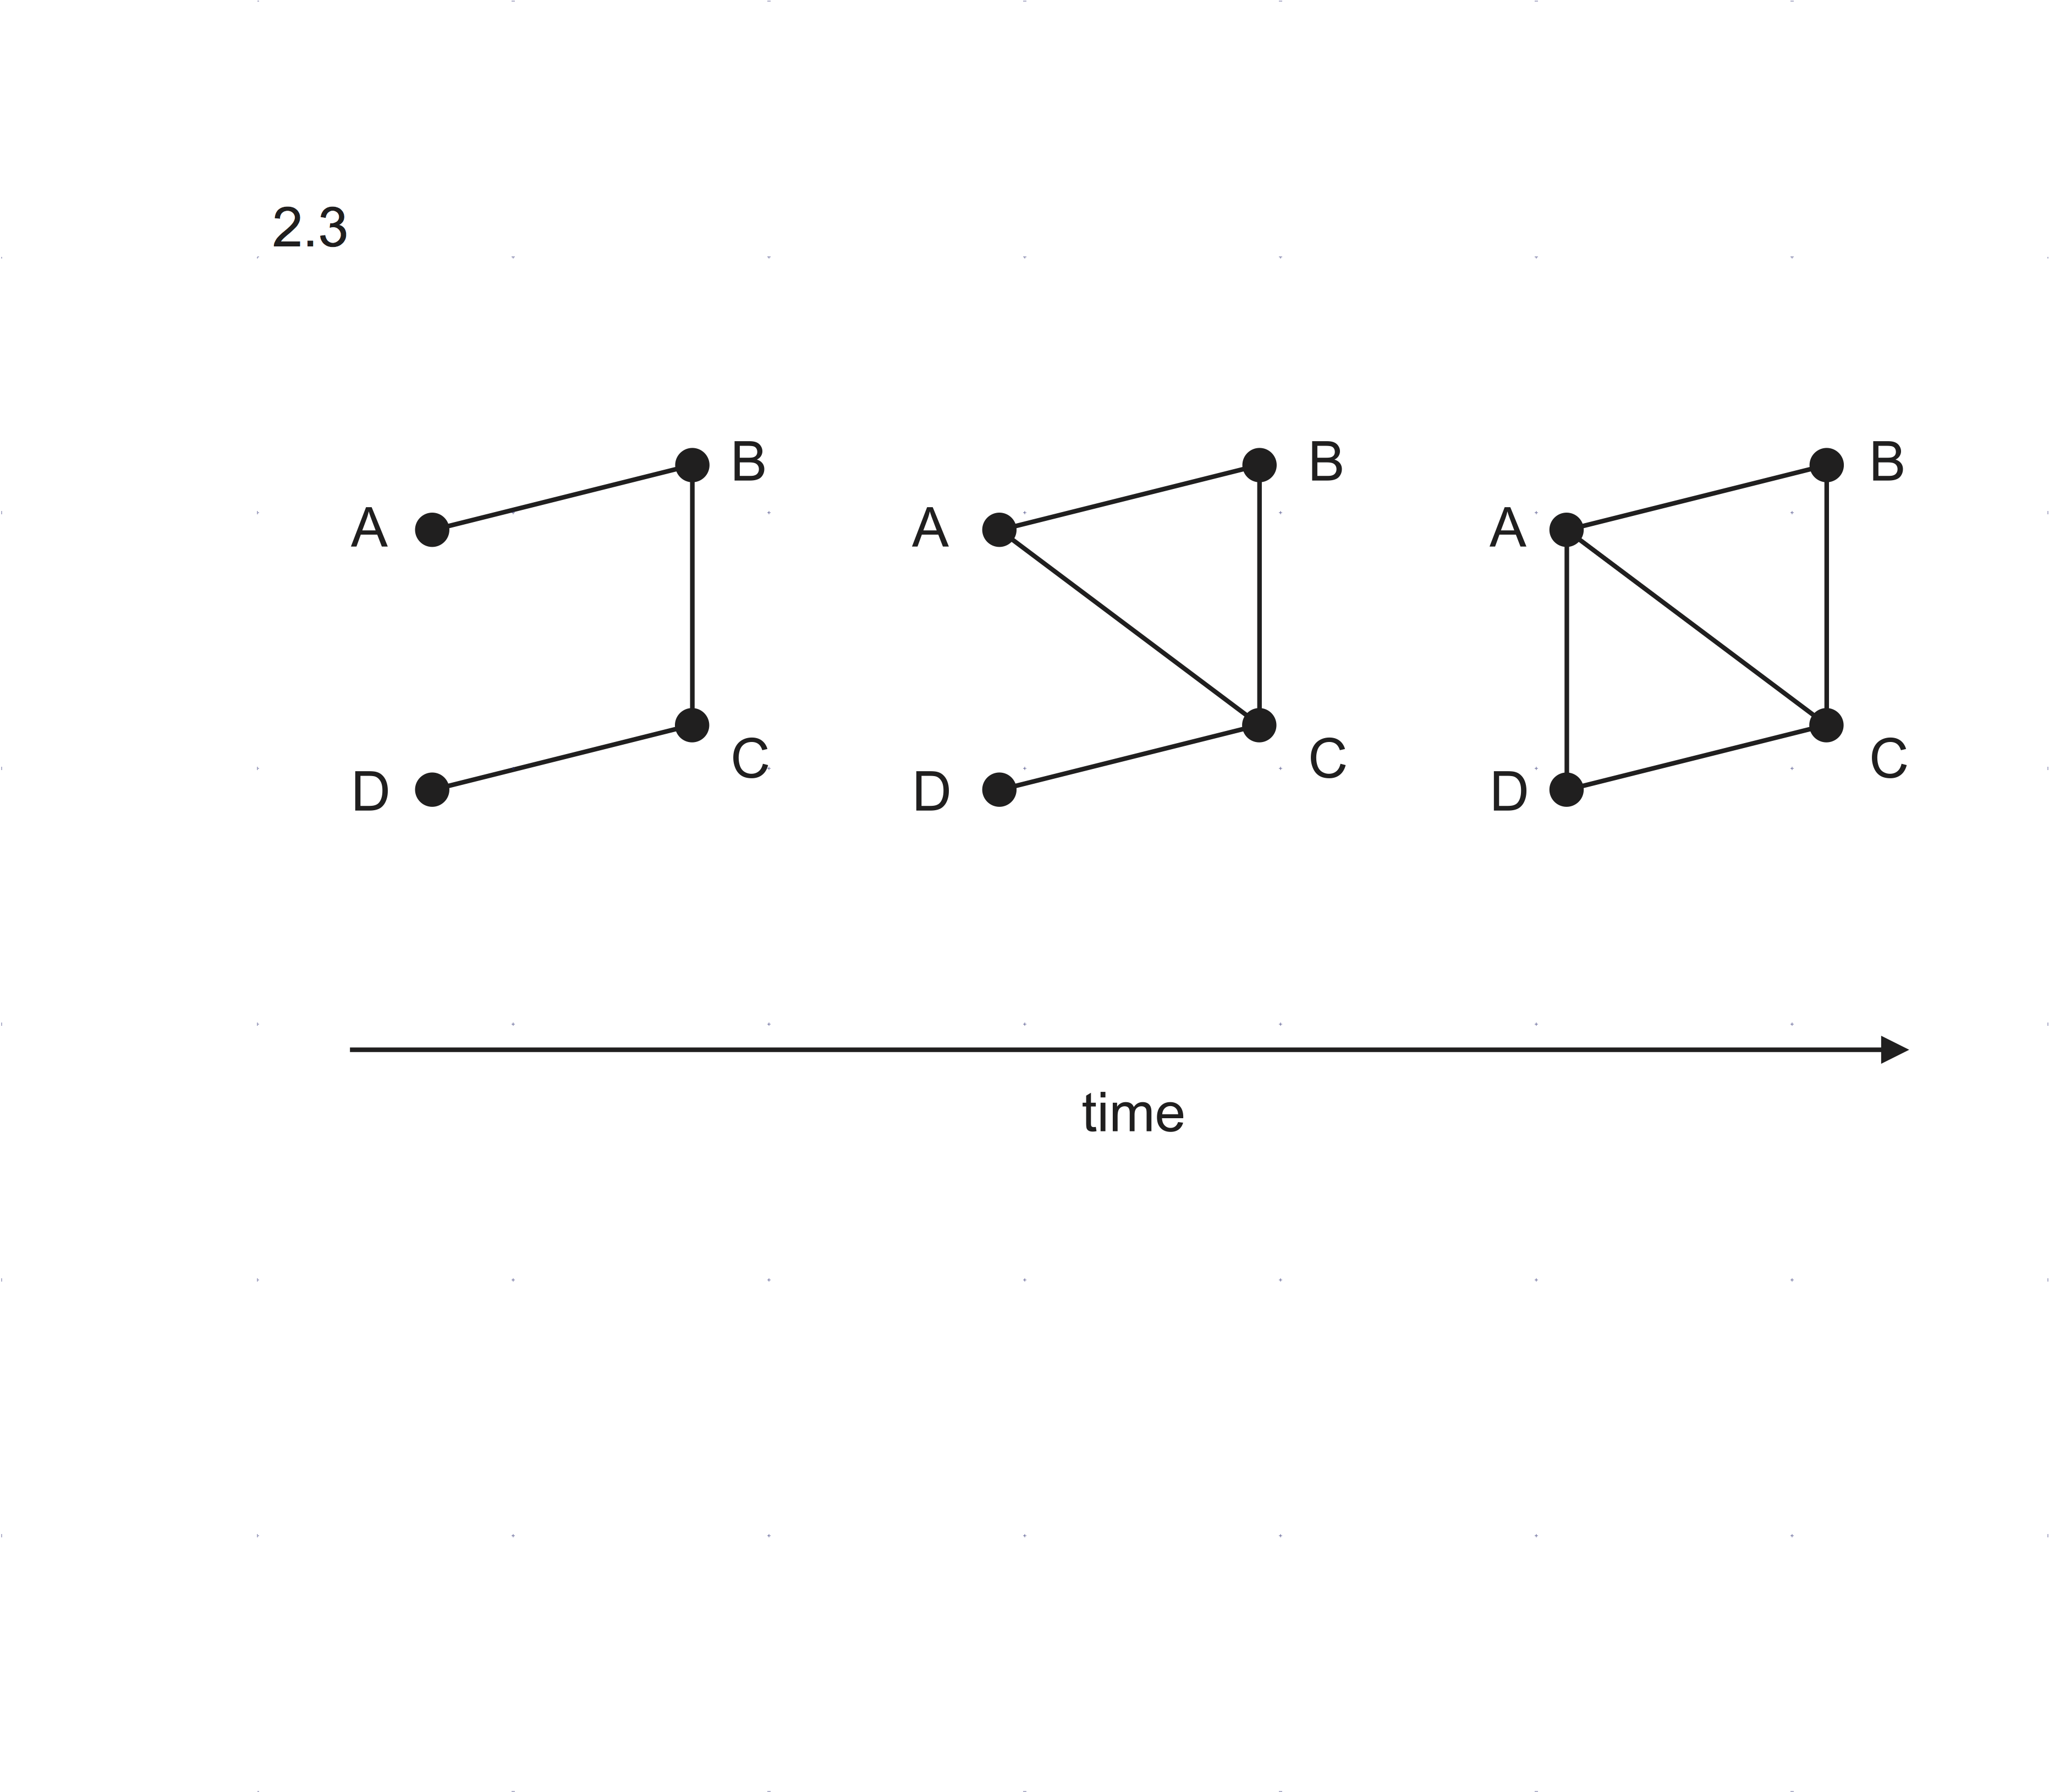
\includegraphics[width=\textwidth]{figures_book/2_3}
\end{figure}

\note{
How do you start? with random graph and fill in edges?  leads to completely connected network.  Duncan and I worked on this problem for one whole summer and got nowhere.\\
}

\end{frame}
%%%%%%%%%%%%%%%%%%%%%%%%%%%%
\begin{frame}

\begin{columns}
\begin{column}{0.6\textwidth}
For a detailed mathematical treatment of random graphs, I recommend:
\end{column}
\begin{column}{0.4\textwidth}
\begin{figure}
\centering
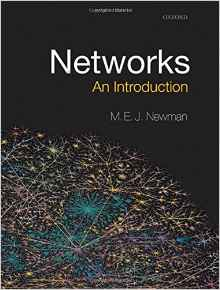
\includegraphics[width=\textwidth]{figures/newman_networks_2010_cover}
\end{figure}
\end{column}
\end{columns}

\end{frame}
%%%%%%%%%%%%%%%%%%%%%%%%%%%%%%%

\end{document}
